\RequirePackage{fix-cm}
\documentclass[smallextended]{svjour3}          % twocolumn

\smartqed  % flush right qed marks, e.g. at end of proof

\usepackage{graphicx} % adjustbox loads it
\usepackage{epstopdf} % loads eps
\usepackage[normalem]{ulem}

% insert here the call for the packages your document requires
\usepackage{geometry}
\usepackage[export]{adjustbox}
\usepackage[labelfont=bf, labelsep=space]{caption}
%\usepackage{subcaption}
\usepackage{subfig}
\usepackage[utf8]{inputenc}
\usepackage{amssymb}
\usepackage{amsmath} 

\usepackage{natbib} % enables author year and other citation styles
\usepackage[bookmarks,bookmarksopen,bookmarksdepth=2]{hyperref} % active links
\hypersetup{backref,
	colorlinks=true,
	citecolor=blue,
	linkcolor=blue}

\usepackage{tikz} % graphics,
\usetikzlibrary{fit,positioning} % tikz elements positioning
\usepackage{soul} % annotations


\DeclareMathOperator*{\argmin}{arg\,min}



\begin{document}

\title{Detection of user roles with thread growth models}
%\subtitle{Do you have a subtitle?\\ If so, write it here}
%\titlerunning{Detection of user roles with thread generative models}        % if too long for running head

\author{Alberto Lumbreras \and
        Julien Velcin  \and\\
        Marie Guégan \and
        Bertrand Jouve
}

%\authorrunning{Short form of author list} % if too long for running head

\institute{Alberto Lumbreras \and Marie Guégan \at
		   Technicolor\\
           975 Avenue des Champs Blancs, \\35576 Cesson-Sévigné,\\ France\\
           \email{alberto.lumbreras@technicolor.com}\\
           \email{marie.guegan@technicolor.com}
           \and
           Julien Velcin \at
           Laboratoire ERIC, Université de Lyon,\\
           5, avenue Pierre Mendès France, 69676 Bron,\\ France\\
           \email{julien.velcin@univ-lyon2.fr}
		  \and
           Bertrand Jouve \at
           Université de Toulouse; UT2; FRAMESPA/IMT; 5 allée Antonio Machado, 31058 Toulouse, cedex 9\\
           CNRS; FRAMESPA; F-31000 Toulouse\\
           CNRS; IMT; F-31000 Toulouse\\ France\\     
           \email{jouve@univ-tlse2.fr}
}

\date{Received: date / Accepted: date}
% The correct dates will be entered by the editor

\maketitle


\section{Introduction}
Random graph models are stochastic generators of graphs that try to reproduce the properties of a some real-world graphs. Ideally, these models should reproduce a large set of properties using a minimum number of assumptions and parameters. If the generated graphs and the real-world graphs share some relevant properties, then the proposed growth mechanism might be a reasonable approximation of the growth laws under which the real-world graphs evolve \citep{Kolaczyk2009}. Formally, a growth model is a probability distribution that quantifies the probability of an existing vertex $i$ of being chosen as the parent for a new vertex $x_t$:
\begin{align*}
p(x_t \sim i | G_{t-1}; \boldsymbol{\theta})
\label{eq:growth_model}
\end{align*} 
where $G_{t-1}$ is the state of the graph before $x_t$ is attached and $\boldsymbol{\theta}$ is the vector of model parameters.

Online discussions can be regarded as evolving tree graphs where vertices represent messages and a directed edge indicates that a message is a reply to another message. The tree starts with the root message that starts the conversation, and then evolves towards some form of tree. Different models have been proposed to account for both the way how a tree evolves and the final properties of the tree. The parameters of these models are fixed and every new vertex is assumed to chose its parent according to the current state of the graph $G_{t-1}$ and a set of fixed parameters that govern the whole process. These parameters regulate, for instance, the tendency to reply to the root, or how fast a vertex with more replies attracts more replies.  Since the parameters are fixed, these models implicitly assume that the choice of a parent is independent of the user who writes the new post.

In this chapter, we explicitly assume that posts written by different users may have different parameters. Some users, for instance, might tend to reply to the root and avoid conversations deeper in the tree. Others might tend to ignore old posts. Others might be specially attracted by popular posts. Formally, we assume that there are $K$ latent types of users and that users of type $k$ behave according to their own group parameters $\boldsymbol{\theta}_k$.  Equation~\ref{eq:growth_model} depends now on the author of post $x_t$:
\begin{align*}
p(x_t \sim i | G_{t-1}; \boldsymbol{\theta}_{z_u})
\end{align*}
where $z_u$ is the group of user $u$ and  $\boldsymbol{\theta}_{z_u}$ are the parameters of that group.

The remaining of this chapters is structure as follows: first, we recall the Preferential Attachment model and we present the thread models. Then we present our model, which finds $k$ sets of parameters for $k$ types of user. Finally, we compare both models and show that, while there is no a remarkable difference on how they reproduce structural properties of real threads, our model can be used for recommendation of posts. 

\begin{figure}
	\subfloat[$p=0.1$]{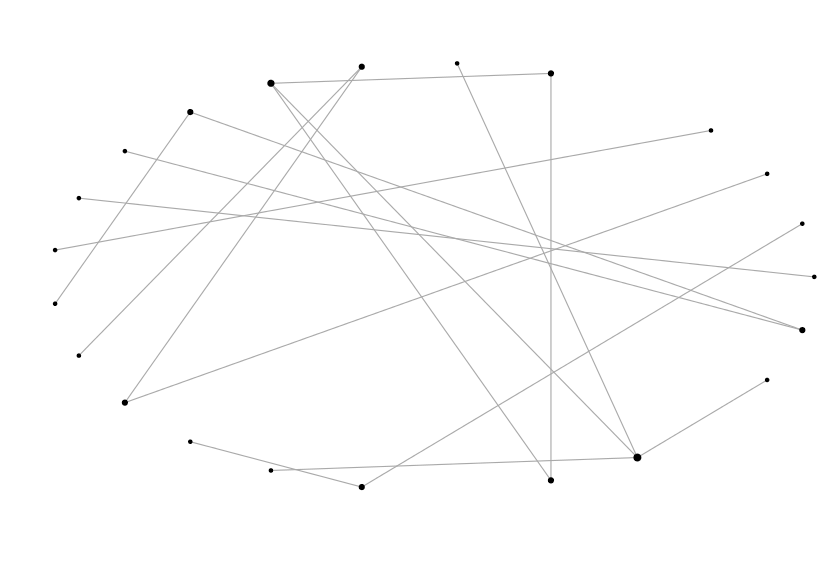
\includegraphics[width=0.33\textwidth]{erdos_01}}
	\subfloat[$p=0.5$]{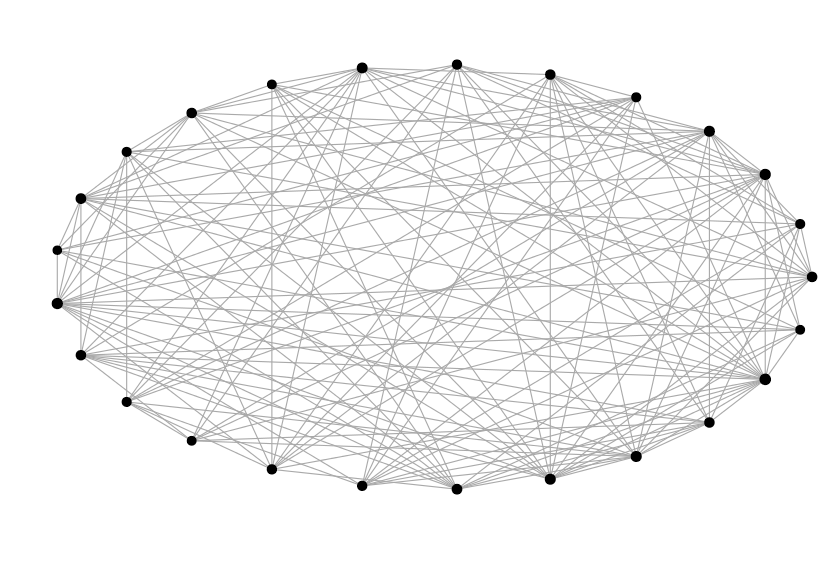
\includegraphics[width=0.33\textwidth]{erdos_05}}
	\subfloat[$p=1$]{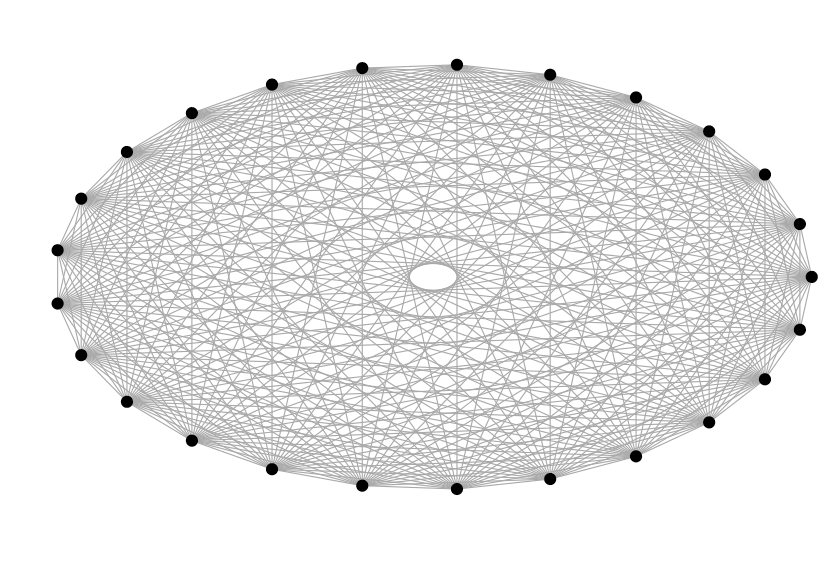
\includegraphics[width=0.33\textwidth]{erdos_1}}
	\caption{Erdös-Rényi graphs}
	\label{fig:erdos_rendy}
\end{figure}


\section{Network Growth model}\label{sec:related-work}

Growth models try to reproduce not only the final properties of the network but also how the network is built. The \textit{preferential attachment} model proposed by \cite{Barabasi1999} is the best well-known member of this family.
The Barabasi-Albert model builds a graph by sequentially adding its vertices; once a new vertex $x$ is added to the graph it decides whether to create an edge to an existing vertex $i$ with probability

\begin{align}
	p(x \sim i | G) =\frac{d_{i}^\alpha}{Z}; &\qquad
	Z = \sum_{j=1}^{|V(G)|} d_j^\alpha
\end{align}
where $d_i$ is the degree of the vertex $i$ before vertex $x$ is added\footnote{To avoid loaded notations we avoid writing $G_{t-1}$ $d_{i,t-1}$ and $Z_{t-1}$ when it is clear by the context that they correspond to the last state of the graph before adding the new node $x$.}. No This model reproduces a rich-get-richer phenomena controlled by the parameter $\alpha$. The particular case of $\alpha=1$ is called \textit{linear preferential-attachment} since the probabilities increase linearly with the number of degrees. Figure~\ref{fig:Barabasi-Albert} shows examples of Barabasi-Albert graphs generated with different $\alpha$. The Barabasi-Albert explains very well the power-law degree distributions observed in many real graphs.

\begin{figure}
	\centering
	\subfloat[$\alpha=0$]{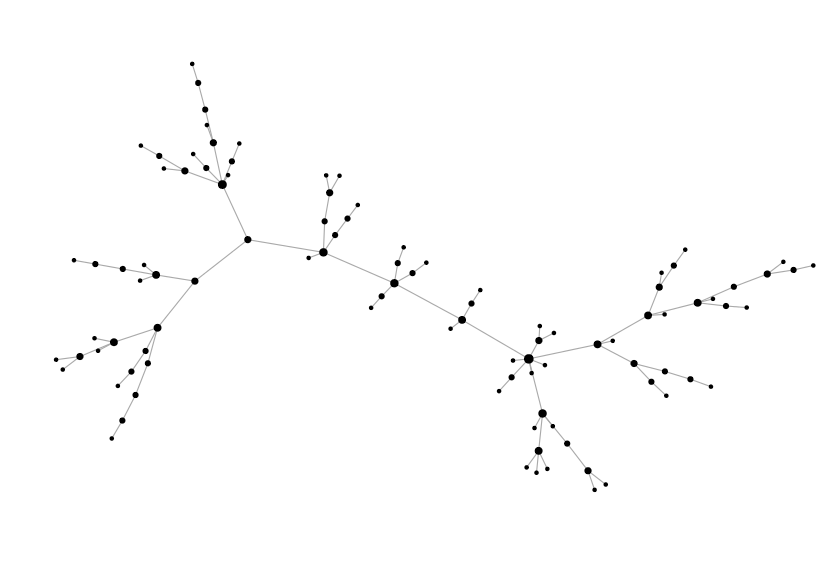
\includegraphics[width=0.33\textwidth]{barabasi_0}}
	\subfloat[$\alpha=1$]{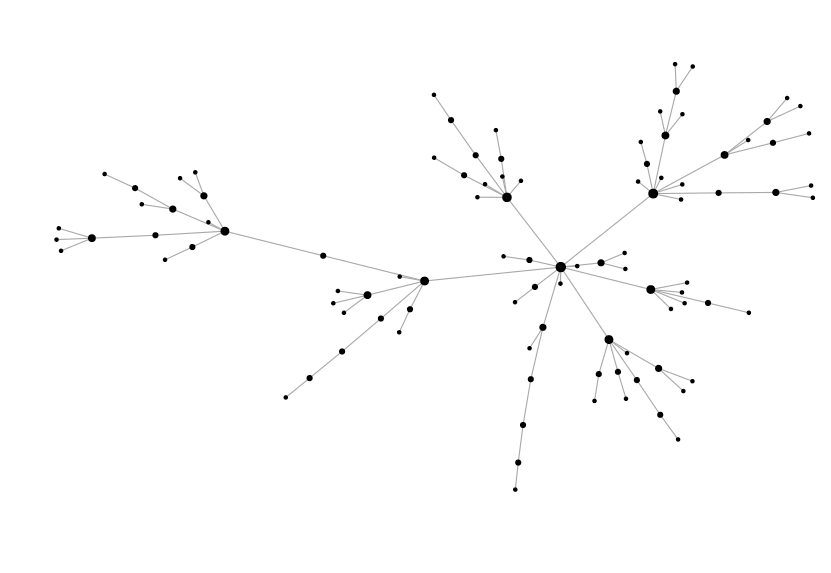
\includegraphics[width=0.33\textwidth]{barabasi_1}}
	\subfloat[$\alpha=1.8$]{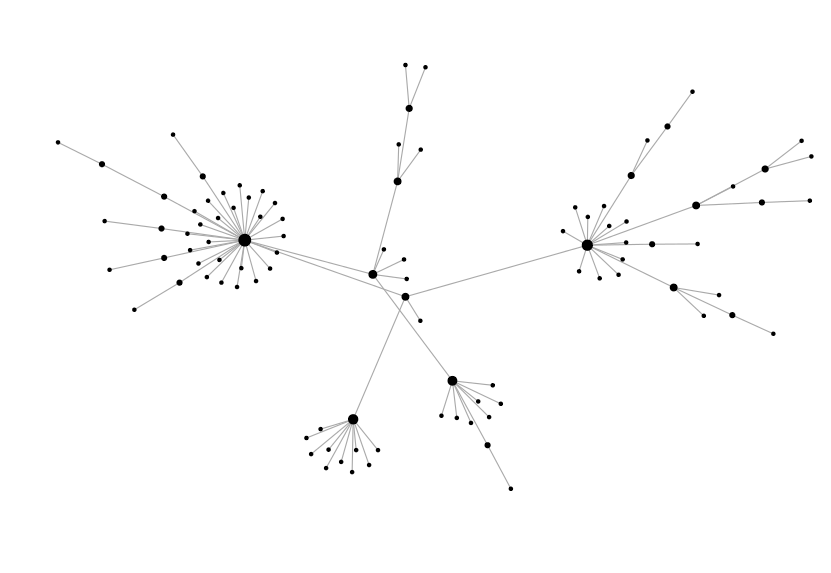
\includegraphics[width=0.33\textwidth]{barabasi_1_8}}
	\caption{Barabasi-Albert graphs with one edge created at every step.}
	\label{fig:Barabasi-Albert}
\end{figure}



During the recent years, some authors have proposed models to explain the growth of online conversations. \citep{Kumar2010, Gomez2010, Wang2012e, Gomez2012}. We describe this models in the following sections.

%%%%%%%%%%%%%%%%%%%%%%%%%%%%
\subsection{Preferential attachment and recency}
\cite{Kumar2010} proposed a model that combines both \textit{preferential-attachment} and \textit{recency}. The higher the degree of a post and the later it was published, the easier for this post to attract the incoming replies. At every time step, a decision is made to stop the thread or to add a new post. Every new post choses its parent according to:
\begin{align}
p(x\sim i | G) = \frac{h(d_u, r_u)}{Z}; \qquad h(d_u, r_u) =\alpha d_u + \tau^{r_u} ; \qquad Z = \sum_{n=1}^{|V(G)|} h(d_n, r_n) + \delta
\end{align}
where $r_u$ is the number of time steps since $u$ was added to the thread. The authors report that when the alternative function $h(d_u, r_u) = d_u \tau^{r_u}$ is used, the recency factor prevents the preferential attachment factor from generating heavy-tailed degree distributions. The choice of placing $\alpha$ as a coefficient instead of an exponent is made for mathematical convenience so that $Z$ does not depend on the graph structure at that particular moment.

The authors also propose an improvement of the model to account for the identity of posts authors. For a new post $v$ replying to a post $u$, its author $a(v)$ can be either $a(u)$ (a self-reply), another author $a(w)$ that has already participated in the chain from $u$ to the root, or some other new author belonging to the set of authors $A$ that have not participated in the chain:
\begin{align}
a(v) = 
\begin{cases}
a(w) & \text{ with probability } \gamma\\
a(u) & \text{ with probability } \epsilon\\
a \in A & \text{ with probability } 1 -\gamma - \epsilon 
\end{cases}
\end{align} 

\subsubsection*{Parameter estimation}
The parameters are estimated by a grid search computing the maximum likelihood estimation of different $\alpha, \tau, \gamma, \epsilon$.

\subsection{Preferential attachment and root bias}
In \cite{Gomez2010} the authors combine \textit{preferential-attachment} with a \textit{bias towards the root}. The probability of choosing an existing parent $k$ is:
\[
%p(\pi_t = k | \boldmath{\pi}_{(1:t-1)}) 
%\propto 
%(\beta_k d_{k,(t-1)})^{\alpha_k}
p(x \sim k | G) 
\propto 
(\beta_k d_{k})^{\alpha_k}
\]
where 
\begin{align}
\alpha_k = 
\begin{cases}
	\alpha_1 & \text{ for } k=1 \\	
	\alpha_c & \text{for } k \in \{2,...,t\}
\end{cases}\notag\\
\beta_k = 
\begin{cases}
\beta & \text{ for } k=1 \\	
1 & \text{for } k \in \{2,...,t\}
\end{cases}
\end{align}
Note that $\alpha_k$ is the preferential attachment exponent and that if $\alpha_1=\alpha_c$ and $\beta=1$ we recover the Barabasi-Albert model of preferential attachment.
\subsubsection*{Parameter estimation}
Maximum Likelihood Estimation of $\alpha_1, \alpha_c$ and $\beta$ is done by minimizing the negative log-likelihood:

%\begin{equation}
%	\log \mathcal{L}(\boldsymbol{\Pi} | \alpha_k, \beta_k)
%	=
%	\sum_{i=1}^{N}
%	\sum_{t=2}^{|\pi_i|}
%	\alpha_k (\log \beta_k+ \log d_{k,1:(t-1)}) 
%	-
%	\log \sum_{l=1}^{t} (\beta_l d_{l,1:(t-1)})
%\end{equation}
\begin{equation}
\log \mathcal{L}(\mathbf{G} | \alpha_k, \beta_k)
=
\sum_{i=1}^{N}
\sum_{t=2}^{|V(G_i|}
\alpha_k (\log \beta_k+ \log d_{k,(t-1)}) 
-
\log \sum_{l=1}^{t} (\beta_l d_{l,(t-1)})
\end{equation}
Since this is a convex function, the minimization is done with the Nelder-Mead algorithm (\texttt{fminsearch} in Matlab).The authors fitted the parameters to several datasets and then generate graphs that resemble the original conversations (see Figure~\ref{fig:Gomez}).

	\begin{figure}
		\centering
		\subfloat[real]{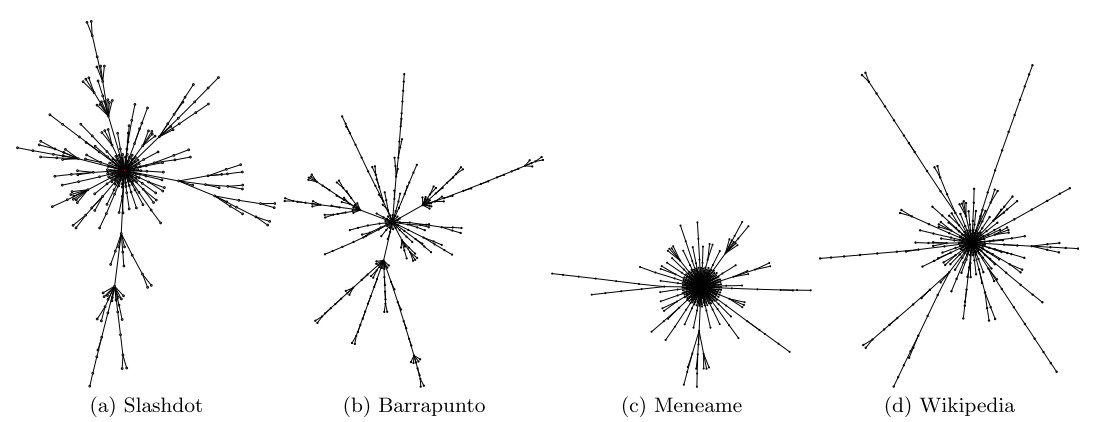
\includegraphics[width=0.45\textwidth]{gomez_real}}\hfill
		\subfloat[synthetic]{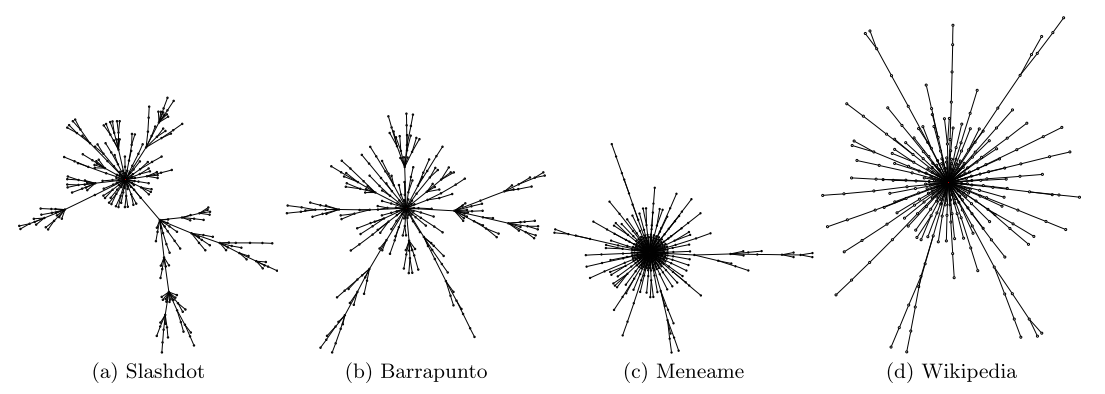
\includegraphics[width=0.45\textwidth]{gomez_synthetic}}
		\caption{Random grahs for discussion threads. Gómez-Kappen-Kaltenbrunner}
		\label{fig:Gomez}
	\end{figure}


\subsection{Preferential attachment, root bias and recency}
In \cite{Gomez2012} the authors combine \textit{preferential-attachment}, a \textit{bias towards the root} and \textit{novelty}. Unlike in their former model in \cite{Gomez2010}, here they sum these factors instead of multiplying them:

\begin{equation}
%p(\pi_t = k | \boldmath{\pi}_{(1:t-1)}) 
%\propto 
%(\beta_k d_{k,(t-1)})^{\alpha_k}
p(x \sim k | G) 
\propto 
\beta_k + \alpha d_{k, (t-1)} + \tau^{t-k}
\end{equation}

\subsubsection*{Parameter estimation}
The negative log-likelihood to be minimized is: 
%\begin{equation}
%	\log \mathcal{L}(\boldsymbol{\Pi} | \alpha_k, \beta_k, \tau)
%	=
%	\sum_{i=1}^{N}
%	\sum_{t=2}^{|\pi_i|}
%	\beta_k+
%	\alpha_k d_{k,1:(t-1)}
%	+ \tau^{t-k+1}	
%\end{equation}
\begin{equation}
\log \mathcal{L}(\mathbf{G} | \alpha, \beta_k, \tau)
=
\sum_{i=1}^{N}
\sum_{t=2}^{|V(G_i)|}
\log
\left(
\beta_k+
\alpha d_{k,(t-1)}
+ \tau^{t-k}
\right)
- \log
\sum_{l=1}^{t}
\left(\beta_l+
\alpha d_{l, (t-1)}
+ \tau^{t-l}
\right)
\end{equation}
As in \cite{Gomez2010}, parameters are optimized through numerical methods.



\subsection{Time-sensitive preferential attachment}
In \cite{Wang2012e} authors make two observations. On the one hand, that distance between its posts follows an upper-truncated Pareto distribution. On the other hand, that threads grow faster when they are featured in the front page (or some sections showing the top discussions at that moment) and they slow down once they disappear from the front page. From this, they propose a model that models the growth of a thread in a given forum. As for the structure, they use preferential-attachment. It is the only existing model that includes real time.

\subsubsection*{Parameter estimation}
Their model has two parts: a upper-truncated distribution to model the time of response and the preferential attachment to model the structure.
Authors use their Maximum Likelihood estimators, which are both known in the literature.

\subsection{Limitations of current models}
There are two aspects that might me improved:

\begin{itemize}
	\item Time is only poorly combined with the structure in \cite{Wang2012e}. Actually in this model time is independent of the structure and vicecersa. As suggested in \cite{Gomez2012} (Conclusions) combining both time and structure is an interesting line of research. Besides, there are probably other ways of consider time.
	
	\item These models estimate their parameters once and therefore very different threads are summarized with common parameters. However, imagine that we learned our parameters from a set of threads $\mathbf{G}$ and now we want to make predictions on a particular new thread $G^*$, that is, we want to compute $p(x \sim i | G_{1:t-1}^*, \mathbf{G})$. There is a lot to be learned from the particular ongoing dynamics of the conversation until time $t$, and making predictions based on the globally estimated parameters will not be flexible enough to adapt the prediction to the last observations. Bayesian inference is a natural way to do this since we will be constantly updating our believes every time a new observation (post) arrives. The challenge here is its computational cost, so we should  
	probably work with fast approximations to the posterior
\end{itemize}
% second goal: predictions
Growth graph models are stochastic processes governed by a set of parameters. Once these parameters are estimated, the model does not change anymore. Yet, threads can vary a lot and therefore the parameters that explain the global dataset do not usually explain the specific dynamics of a particular discussion. 

\section{Mixture-based model}

We build our model over \cite{Gomez2012}. We consider the there are $N$ latent groups of users and that each group $i$ has its own parameters $\alpha_i, \beta_i, \tau_i$. Our task is to detect the latent clusters and the parameters associated to each cluster. For this, we will make use of the Expectation-Maximization algorithm.

\subsection{General EM} 

\begin{align}
\ln p(\mathbf{X} | \boldsymbol{\theta}) &=  \ln \sum_{\mathbf{Z}}  p(\mathbf{X}, \mathbf{Z}  | \boldsymbol{\theta}) \\
&=\ln \sum_{\mathbf{Z}} q(\mathbf{Z}) \frac{p(\mathbf{X}, \mathbf{Z}  | \boldsymbol{\theta})}{ q(\mathbf{Z})}\\
&\geq \sum_{\mathbf{Z}} q(\mathbf{Z}) \ln \frac{p(\mathbf{X}, \mathbf{Z} | \boldsymbol{\theta)}}{q(\mathbf{Z})}
\end{align}


The equality holds when $q(\mathbf{Z})$ is the posterior $p(\mathbf{Z} | \mathbf{X}, \boldsymbol{\theta})$:
\begin{align}
\ln p(\mathbf{X} | \boldsymbol{\theta}) &=  \sum_{\mathbf{Z}} p(\mathbf{Z} | \mathbf{X}, \boldsymbol{\theta}) \ln \frac{p(\mathbf{X, Z} | \boldsymbol{\theta})}{ p(\mathbf{Z} | \mathbf{X}, \boldsymbol{\theta})} \qquad \blacksquare
\label{eq:em_general}
\end{align}


\subsection{EM for current model} 

Given a post $n$ written at time step $t$, we consider the three following observations: the degree of its parent at time $t-1$, denoted as $d_n$; whether its parent is the root post, denoted as $r_n$; and the lag, in time steps, between the post and its parent, denoted as $l_n$. Let $\mathbf{X} = \{x_1,...,x_N\}$ be a matrix where $x_i = \{t_i, d_i, r_i, l_i\}$

The model of \cite{Gomez2012} can be expressed as:

\begin{align}
p(\mathbf{X} | \boldsymbol{\theta}) = \prod_{n=1}^N
\frac{\alpha d_n + \beta r_n + \tau^{l_n}}{\alpha(t_n-1)+\beta + \frac{\tau(\tau^{t_n}-1)}{\tau-1}}
\end{align} 

where instead of looping through all the posts in all the trees, we just look through all the posts. The reason to change the notation is that this will make or equations more uncluttered, it makes it more universal (the total likelihood expressed a single product individual likelihoods), and that is friendlier to code, since we think of the data as a matrix rather than as a set of trees .  

We consider that there exists latent groups of users where every group has its own parameters $\mathbf{\theta}_k = \{\alpha_k, \beta_k, \tau_k\}$. Our task, then, is to estimate the parameters of each group and the group where each user belongs. Let $\mathbf{X}_u$ the submatrix of $\mathbf{X}$ composed of all posts written by user $u$. Let $\mathbf{Z} = \{z_1,...,z_U\}$ be the indicators matrix where $z_i=\{z_{i1},...,z_{iK}\}$ and where $z_{ik}$ is one if user $i$ belongs to group $k$ and zero otherwise.    


In the following, we will prepare the elements needed in Equation~\ref{eq:em_general}. First, we need the complete loglikelihood. The complete likelhood is:
\begin{align}
p(\mathbf{X, Z} | \boldsymbol{\theta}) &= 
\prod_{n=1}^N \prod_{k=1}^K \pi_k^{z_{nk}}
\left(
\frac{\alpha_k d_n + \beta_k r_n + \tau_k^{l_n}}{\alpha_k(t_n-1)+\beta_k + \frac{\tau_k(\tau_k^{t_n}-1)}{\tau_k-1}}
\right)^{z_{nk}}
\end{align}
and its logarithm:
\begin{align}
\ln p(\mathbf{X, Z} | \boldsymbol{\theta}) &= 
\sum_{n=1}^N \sum_{k=1}^K z_{nk}
\left(\ln \pi_k + 
ln \frac{\alpha_k d_n + \beta_k r_n + \tau_k^{l_n}}{\alpha_k(t_n-1)+\beta_k + \frac{\tau_k(\tau_k^{t_n}-1)}{\tau_k-1}}\right)
\end{align}
Note that we use indicator variables for the posts to avoid introducing the users for now. A post has the indicator of the user who wrote it. On the other hand, the posterior distribution of the latent factors is:
\begin{align*}
p(\mathbf{Z} | \mathbf{X}, \boldsymbol{\theta}) 
\propto 
p(\mathbf{X,Z} | \boldsymbol{\theta})
\end{align*}
that can be factorized in $\mathbf{z}_1,...\mathbf{z}_U$. For a given user $u$:
\begin{align*}
p(z_u | \mathbf{X}_u, \boldsymbol{\theta}) 
\propto 
p(\mathbf{X}_u, z_u | \boldsymbol{\theta})
\end{align*}

The expected value of the indicator variable $z_uk$ under this posterior distribution is given by:
\begin{align}
\mathbb{E}[z_{uk}] 
&= 
\frac{\sum_{z_u} z_{uk} \prod_c\left[\pi_c \frac{\alpha_c d_n + \beta_c r_n + \tau_c^{l_n}}{\alpha_c(t_n-1)+\beta_c + \frac{\tau_c(\tau_c^{t_n}-1)}{\tau_c-1}} \right]^{z_{uc}}}
{\sum_{z_u} \prod_c\left[\pi_c \frac{\alpha_c d_n + \beta_c r_n + \tau_c^{l_n}}{\alpha_c(t_n-1)+\beta + \frac{\tau_c(\tau_c^{t_n}-1)}{\tau_c-1}} \right]^{z_{uc}}}
=
\frac{\pi_{k} \frac{\alpha_c d_n + \beta_c r_n + \tau_c^{l_n}}{\alpha_c(t_n-1)+\beta_c + \frac{\tau_c(\tau_c^{t_n}-1)}{\tau_c-1}}}
{
\sum_{j=1}^{K}\pi_{j} \frac{\alpha d_n + \beta r_n + \tau^{l_n}}{\alpha(t_n-1)+\beta + \frac{\tau(\tau^{t_n}-1)}{\tau-1}} 
}
= \gamma(z_{uk})
\end{align}
\footnote{TODO: This has to be done by user, not by post. there is a product missing. Actually use logs, sum and finally get back with exp}
Finally, we can obtain the expected value of the complete data log likelihood:
\begin{align}
\mathbb{E}_{\mathbf{Z}}[\ln p(\mathbf{X,Z} | \boldsymbol{\theta})] &=
\sum_{n=1}^N \sum_{k=1}^K \gamma(z_{nk})
\left(
\ln \pi_k + 
ln \frac{\alpha_k d_n + \beta_k r_n + \tau_k^{l_n}}{\alpha_k(t_n-1)+\beta_k + \frac{\tau_k(\tau_k^{t_n}-1)}{\tau_k-1}}
\right)
\end{align}

which we can optimize iteratively.
\newpage
%\appendix
\section*{Appendices}
(Only for internal discussion)

%\bibliographystyle{chicago} % or plain
\bibliographystyle{spbasic} 
\bibliography{bibliography}
\end{document}